\chapter{Исследовательская часть}

В данном разделе будут приведены примеры работы программы, поставлено исследование по сравнению времени синтеза изображения по количеству созданных частиц, а также исследование по сравнению времени синтеза изображения на разном количестве потоков и разном количестве частиц.

\section{Технические характеристики}

Технические характеристики устройства, на котором выполнялось исследование:

\begin{itemize}[label=---]
	\item операционная система Windows 10 Корпоративная, Версия	21H1, Сборка ОС 19043.2006;
	\item память 8 ГБ;
	\item процессор AMD Ryzen 5 4600H с видеокартой Radeon Graphics 3.00 ГГц \cite{processor}.
\end{itemize}

Исследование проводилось на ноутбуке, включенном в сеть электропитания. Во время исследования ноутбук был нагружен только встроенными приложениями окружения, а также непосредственно системой.

\section{Исследование по сравнению времени синтеза изображения по количеству созданных частиц}

Исследование времени синтеза изображения при создании сцен различной нагруженности. Нагрузка будет меняться в зависимости от количества частиц, из которых состоит дым при разном количестве потоков.

Замеры времени синтеза изображения выполнены при помощи класса Stopwatch \cite{csharplangtime}. Предоставляет набор методов и свойств, которые можно использовать для точного измерения затраченного времени.

Замеры времени для каждого количества частиц проводились 50 раз. В качестве результата взято среднее время синтеза изображения на данном количестве частиц. на данном количестве потоков.

Результаты замеров приведены в таблицах \ref{tbl:compare} и на рис. \ref{fig:compare}.

\captionsetup{justification=raggedright, singlelinecheck=false}
\begin{table}[H]
	\caption{Зависимость производительности от количества частиц}
	\label{tbl:compare}
	\begin{center}
		\begin{tabular}{|c|d|}
			\hline
			Частиц, штук & \multicolumn{1}{c|}{Время синтеза, мс}\\ \hline
			1000&	3609.8\\ \hline
			2000&	7054.9\\ \hline
			3000&	10667.4\\ \hline
			4000&	14087.2\\ \hline
			5000&	17562.4\\ \hline
			6000&	21814.1\\ \hline
			7000&	25446.5\\ \hline
			8000&	29256.9\\ \hline
			9000&	33760.7\\ \hline
			10000&	37528.8\\ \hline
			11000&	41513.6\\ \hline
			12000&	47304.2\\ \hline
			13000&	50515.8\\ \hline
			14000&	54719.8\\ \hline
			15000&	63106.3\\ \hline
		\end{tabular}
	\end{center}
\end{table}

\captionsetup{justification=centering}

\begin{figure}[H]
	\centering
	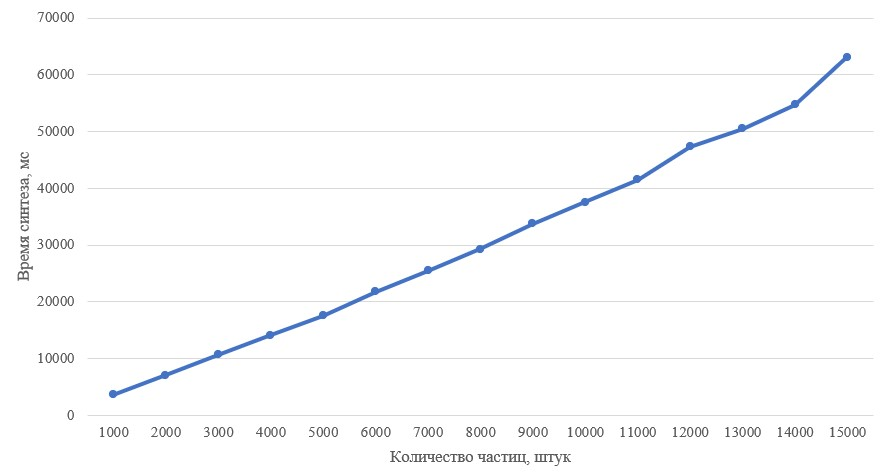
\includegraphics[width=1\linewidth]{inc/img/compare}
	\caption{Зависимость времени синтеза изображения от количества частиц на сцене}
	\label{fig:compare}
\end{figure}

Как видно из результатов, время синтеза изображения увеличивается линейно при линейном увеличении количества частиц в дыме. 

\section{Исследование по сравнению времени синтеза изображения на разном количестве потоков и разном количестве частиц}

Результаты замеров приведены в таблице \ref{tab:time}.
На рисунке \ref{fig:compfig} приведена зависимость времени работы реализации алгоритма от количества потоков и количества частиц в дыме.
\captionsetup{justification=raggedright,singlelinecheck=false}
\begin{table}[H]
	\begin{center}
		\caption{\label{tab:time}Время выполнения реализации алгоритма обратной трассировки лучей при количества потоков и количества частиц в дыме}
		\begin{tabular}{|c|d|d|d|d|d|}
			\hline				
			\multirow{3}{*}{\makecell{Количество\\ частиц,\\ штук}} & 	\multicolumn{5}{c|}{Количество потоков, штук} \\ [3ex]
			\cline{2-6}		
			&6&	12&	24&	48&	96\\
			\hline		
			0&	1042.34&	846.74&	948.4&	1060.27&	1100.81\\
			\hline		
			100&	4296.44&	3985.65&	4652.67&	5525.89&	8310.33\\
			\hline		
			200&	7452.28&	6961.98&	7774.77&	9657.25&	15114.46\\
			\hline		
			300&	10535.29&	9723.64&	10917.22&	13735.63&	21985.89\\
			\hline		
			400&	13554.05&	12617.40&	14056.36&	17697.46&	28090.16\\
			\hline		
			500&	16598.27&	15430.81&	17155.82&	21554.69&	34441.75\\
			\hline		
			600&	19478.49&	18153.36&	20216.83&	25357.24&	40506.90\\
			\hline		
			700&	22439.01&	20859.34&	23142.67&	28801.52&	46301.25\\
			\hline		
			800&	25183.41&	23443.41&	26192.44&	32830.08&	51871.79\\
			\hline		
			
		\end{tabular}
	\end{center}
\end{table}
\captionsetup{justification=centering,singlelinecheck=false}
\begin{figure}[H]
	\centering
	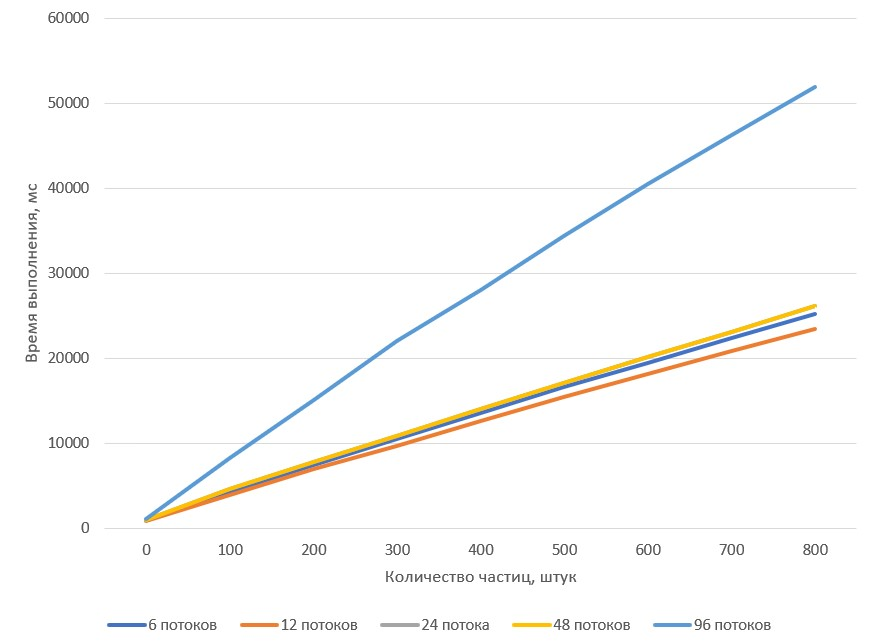
\includegraphics[width=0.9\linewidth]{inc/img/comp_fig}
	\caption{Зависимость времени выполнения реализации алгоритма обратной трассировки лучей от количества потоков и количества частиц в дыме}
	\label{fig:compfig}
\end{figure}

При 12 потоках достигается пик, при котором все логические ядра процессора одновременно выполняют трассировку лучей. Далее при увеличении числа потоков производительность падает. Это объясняется тем, что создается очередь потоков, которая замедляет работу программы.

\section*{Вывод}

В данном разделе были рассмотрены примеры работы программного обеспечения, а также выяснено в результате эксперимента, что время синтеза изображения увеличивается линейно при линейном увеличении количества частиц.

